\documentclass[a4paper,review,12pt,authoryear]{elsarticle}

\usepackage{natbib}
\usepackage{amsfonts,amsmath,bm,xcolor, booktabs,hyperref}
\usepackage[ruled]{algorithm2e}
\usepackage{geometry}
\usepackage{subfig}
\geometry{a4paper,scale=0.8}
\usepackage{setspace}
\setstretch{1.5}
\let\code=\texttt
\let\proglang=\textsf
\setcounter{MaxMatrixCols}{20}


\newcommand{\bY}{\mathbf{Y}}
\newcommand{\bpi}{\bm{\pi}}
\newcommand\independent{\protect\mathpalette{\protect\independenT}{\perp}}
\def\independenT#1#2{\mathrel{\rlap{$#1#2$}\mkern2mu{#1#2}}}

\begin{document}

\begin{frontmatter}

  \title{Discrete forecast reconciliation}

  \author[label1]{Bohan Zhang}
  \address[label1]{School of Economics and Management, Beihang University, Beijing, China}
  
  \author[label1]{Yanfei Kang}
  \author[label2]{Anastasios Panagiotelis}
  
  \author[label3]{Feng Li\corref{cor1}}
  \ead{feng.li@cufe.edu.cn}

  \cortext[cor1]{Correspondance: Feng Li, School of Statistics and Mathematics, Central University of Finance and Economics, Shahe Higher Education Park, Changping District, Beijing 102206, China.}
  \address[label2]{The University of Sydney Business School, NSW 2006, Australia}
  \address[label3]{School of Statistics and Mathematics, Central University of Finance and Economics, Beijing, China}

  \begin{abstract}
    Placeholder for abstract.
  \end{abstract}

  \begin{keyword}
  Forecasting\sep
  Hierarchical time series \sep
  Count data
  \end{keyword}
  
\end{frontmatter}

\newpage

\section{Introduction}

Hierarchical time series is of great concern in many applications, such as supply chain management (\citealp{babaiDemandForecastingSupply2022}), tourism management (\citealp{kourentzesCrosstemporalCoherentForecasts2019}), energy (\citealp{nystrupTemporalHierarchiesAutocorrelation2020}), and mortality (\citealp{liHierarchicalMortalityForecasting2022}).
In the past decades, hierarchical forecasting has attracted significant attention from the forecasting community, yielding many innovative approaches, such as the well-known optimal reconciliation framework (\citealp{hyndmanOptimalCombinationForecasts2011, wickramasuriyaOptimalForecastReconciliation2019, panagiotelisProbabilisticForecastReconciliation2022}) and its variants (\Citealp{zhangOptimalReconciliationImmutable2022a, wickramasuriyaOptimalNonnegativeForecast2020}), deep learning based approaches (\citealp{rangapuramEndtoEndLearningCoherent2021}).
These state-of-art approaches have shown the ability to produce coherent and potentially more accurate forecasts.

Non-negative count time series, especially low-count ones, naturally arise in various areas. 
Examples include intermittent demand in the retail industry (\citealp{kourentzesElucidateStructureIntermittent2021}), the number of 'black swan' events in a period (\citealp{nikolopoulosWeNeedTalk2020}) and violent crimes in one block.
Hierarchical count time series are naturally constructed when decisions in multiple cross-sectional or temporal aggregation levels must be made.
However, most existing hierarchical approaches are intrinsically designed for time series taking continuous values and can not be directly applied to non-negative low-count time series. 
This paper aims to fill this gap and propose a discrete reconciliation approach to produce coherent forecasts for low-count hierarchical time series.

While point and interval forecasts are most widely applied in practice, 
the probability distribution that describes the full uncertainty of future events plays a critical role in optimal decision making. (\citealp{gneitingProbabilisticForecasting2014}) 
With regard to forecasting count time series, it is natural to produce probabilistic forecasts based on predictive mass functions (pmf). 
The pmfs can provide probabilities for each point in their discrete support,
which is especially crucial for low-count time series. (\citealp{petropoulosForecastingTheoryPractice2022a})
By utilizing pmfs, we build a solid fundamental for the proposed discrete reconciliation framework, which is used to define the coherence and incoherence of hierarchical forecasts.

The core objective of hierarchical forecasting is to produce \textit{coherent} forecasts, 
in the sense that point forecasts of a parent series should equal the sum of the point forecasts of associated children series. 
Regarding probabilistic forecasts, the same discipline is applied to each point in the support of hierarchical joint distribution.
Historically, this was achieved by first producing forecasts in one level, 
and then aggregating or disaggregating the forecasts into other levels (\citealp{fliednerHierarchicalForecastingIssues2001}). 
An alternative approach proposed by \cite{hyndmanOptimalCombinationForecasts2011} and further explored by \cite{wickramasuriyaOptimalForecastReconciliation2019}, \cite{ anagiotelisForecastReconciliationGeometric2021}, et al, 
first independently generate \textit{base} forecasts for each time series, 
which are then ``optimally'' reconciled to produce coherent forecasts.

While the reconciliation framework was initially proposed to reconcile point forecasts, it has been extended to probabilistic forecasting. 
The earlier approaches construct coherent probabilistic forecasts by reconciling samples drawn from base forecasts. 
The generated empirical distribution is hence coherent because all the samples are coherent.
\cite{jeonProbabilisticForecastReconciliation2019} propose a method that first draws samples from the independently modelled predictive distribution. 
They then use three alternative approaches, i.e., stacking, ranking and permutation, to construct base forecasts. 
The base forecasts are then reconciled using the reconciliation matrix obtained through cross-validation. 
On the other hand, \cite{bentaiebHierarchicalProbabilisticForecasting2020} construct coherent samples through the bottom-up approach, 
where the dependence among bottom time series is restored using empirical copula modelling.
Furthermore, \cite{panagiotelisProbabilisticForecastReconciliation2022} propose a formal framework for probabilistic reconciliation based on the concept of probabilistic coherence. 
They also propose an efficient algorithm to compute reconciliation weights by optimising a proper scoring rule. 

The forecast reconciliation framework has been proven to enhance forecasting accuracy in various scenarios. 
One of the critical elements of its superior performance should be forecast combination (\citealp{hollymanUnderstandingForecastReconciliation2021}). 
Every reconciled forecast is the weighted combination of all base forecasts,
which could incorporate any external information using arbitrary forecasting methods.
More importantly, the reconciliation process avoids the requirement for complex models that simultaneously capture hierarchical constraints, external information, and serial dependence.
Against this backdrop, the reconciliation framework is a reasonable choice for forecasting hierarchical count time series,
allowing for the employment of existing forecasting approaches for univariate counts in the literature.

To the best of our knowledge, little literature deals with hierarchical count time series forecasting, and none of them is tailored for low-count time series.
\cite{coraniProbabilisticReconciliationCount2022} propose a novel reconciliation approach by conditioning base probabilistic forecasts of the most disaggregated series on base forecasts of aggregated series. 
The reconciled forecasts are obtained through a generalisation of Bayes’ rule and Monte Carlo samplings.
\cite{zambonEfficientProbabilisticReconciliation2022} further generalise this idea to apply for both count time series and real-valued time series.
Although this novel approach produces coherent probabilistic forecasts, 
the conditional manner used is unable to restore the dependence structure within hierarchical time series.
Incorporating correlation requires joint distributions of disaggregated time series, which, as explained above, is challenging to obtain in practice.

In this paper, we seek to address the hierarchical forecasting problem for count time series, especially for low-count time series.
First, we propose the concept of ``coherence'' for hierarchical counts, 
which is similar in some ways to the probabilistic coherence proposed by \cite{panagiotelisProbabilisticForecastReconciliation2022}.
Second, we utilise these concepts to construct a formal reconciliation framework for hierarchical counts, which generally reconciles the forecasts by moving probabilities from incoherent domains to coherent domains.
Third, we show a metric that can be used to evaluate the forecasts and propose an algorithm to optimise this metric. 
To speed up the computation, we further propose a step-wise algorithm based on some reasonable assumptions.
We also show how this algorithm can be solved through quadratic programming.
Fourth, two simulation experiments are performed to verify the applicability 
in both temporal and cross-sectional settings.
Finally, we conduct two empirical experiments to validate its usability in practice further. The first experiment uses a temporal crime dataset, and the other is performed on cross-sectional mortality data.

The remainder of this paper is organised as follows. 
Section \ref{sec:coherence} introduce the notation and the concept of coherence for hierarchical counts.
Section \ref{sec:method} describes the proposed discrete reconciliation framework, the metric used to evaluate the forecasts and the algorithm to reconcile the probabilistic forecasts. 
The step-wise algorithm is also introduced in this section.
Section \ref{sec:simulation} performs two simulation experiments in cross-sectional and temporal settings, and the two empirical experiments are conducted in Section \ref{sec:applications}. Finally, Section \ref{sec:conclusion} concludes with some discussion and thoughts on future research.



\section{Coherence of probabilistic hierarchical count forecasts}

\label{sec:coherence}

	\subsection{Preliminaries}
	Let $\bY=\left(Y_1,Y_2,\ldots,Y_n\right)'$ be an $n$-vector of discrete random variables.
  Let $\bY$ be partitioned so that the first $m$ elements are \textit{base} variables the remaining $(n-m)$ elements are \textit{determined} variables.
  The determined variables are some deterministic linear function of the base variables, usually aggregations. 
  Let the domain of each element of $\bY$ be given by $\mathcal{D}(Y_i)=\left\{0, 1,2,3,\dots,D_i\right\}$, where $D_i$ is finite.
	
	\subsection{Incoherent and Coherent Domain}
	The \textit{incoherent domain} of $\bY$ is given by
	\[
	\hat{\mathcal D}(\bY)=\prod\limits_{i=1}^n\hat{\mathcal D}(\bY_i)=\left\{0, 1,2,\dots,D_1\right\}\times\left\{0,1,2,\dots,D_2\right\}\times\dots\times\left\{0,1,2,\dots,D_n\right\}\,,
	\] 
  where products are set products. The cardinality of the incoherent domain is $|\hat{\mathcal D}(\bY)|=\prod\limits_{i=1}^{n} (D_i+1)$ which will be denoted by $q$. 
  The incoherent domain is analogous to $\mathbb{R}^n$ is the continuous case.
    
  The \textit{coherent domain} of $\bY$ is given by a subset of $\tilde{\mathcal D}(\bY)$ for which aggregation constraints hold.  
  The coherent domain has cardinality $|\tilde{\mathcal D}(\bY)|=\prod\limits_{i=1}^{m} (D_i+1)$. This will be denoted as $r$. 
  The coherent domain is analogous to the coherent subspace $\mathfrak{s}$ in the continuous case (\citealp{panagiotelisProbabilisticForecastReconciliation2022}).
    
    \subsubsection*{Example}
    \label{sec:example}
    
    Let $Y_1$ and $Y_2$ be binary variables and $Y_3=Y_1+Y_2$. In this case the domain of each variable is
    \begin{align*}
      \mathcal{D}(Y_1)=&\left\{0,1\right\}\\
      \mathcal{D}(Y_2)=&\left\{0,1\right\}\\
      \mathcal{D}(Y_3)=&\left\{0,1,2\right\}\,,
    \end{align*}	
    the incoherent domain is
    \begin{align*}
    \hat{\mathcal D}(\bY)=&\left\{\textcolor{blue}{(0,0,0)'},(0,1,0)',(1,0,0)',(1,1,0)',\right.\\
    &\left.(0,0,1)',\textcolor{blue}{(0,1,1)'},\textcolor{blue}{(1,0,1)'},(1,1,1)',\right.\\
    &\left.(0,0,2)',(0,1,2)',(1,0,2)',\textcolor{blue}{(1,1,2)'}\right\}\,,
    \end{align*}
    and the coherent domain is given by those points for which $y_1+y_2=y_3$, highlighted in blue above, i.e
    \[
        \tilde{\mathcal D}(\bY)=\left\{(0,0,0)',(0,1,1)',(1,0,1)',(1,1,2)'\right\}\,.
    \]
    
    \subsection{Coherence of Probabilistic Forecasts}

    Suppose a probabilistic $h$-step ahead forecast is made for $\bY$ at time $t$. 
    Let $\hat{\bpi}^{t+h|t}$ be a $q$-vector of probabilities where each element in $\hat{\bpi}^{t+h|t}$ corresponds to one point in the incoherent domain. 
    Two notational conventions will be used for the elements of $\hat{\bpi}^{t+h|t}$. 
    First, $\hat{\pi}_j^{t+h|t}$ will be used to denote the $j^{th}$ element of $\hat{\bpi}^{t+h|t}$.  
    Second, $\hat{\pi}_{(y_1 y_2 \dots y_n)}^{t+h|t}$ will be used to denote that the specific element of $\hat{\bpi}^{t+h|t}$, corresponds to the forecast probability that the $\bY$ takes a value $(y_1,y_2,\dots,y_n)'$. The two conventions are linked by a function $\hat{h}:{1,2,\dots,q}\rightarrow\hat{\mathcal{D}}(\bY)$ which maps each index $j$ to a configuration of values that $\bY$ can take. 
    Using the small example in the previous section $\hat{\pi}_1^{t+h|t}=\hat{\pi}_{(000)}^{t+h|t}$, $\hat{\pi}_2^{t+h|t}=\hat{\pi}_{(010)}^{t+h|t}$, etc., and $\hat{h}(1)=(0,0,0)'$, $\hat{h}(2)=(0,1,0)'$, etc.
    
    This probabilistic forecast is incoherent as long as there is some $\hat{\bpi}^{t+h|t}_j\neq 0$ for which $\hat{h}(j)\notin\tilde{\mathcal{D}}(\bY)$, i.e. probability is assigned to some points for which the aggregation constraints do not hold. 
    This can happen quite easily in practice. Suppose probabilistic forecasts are generated for each variable independently and the joint forecast is then constructed assuming independence. 
    Such forecasts will in general be incoherent. 
    For example suppose $Pr(Y_1=0)=0.2$,$Pr(Y_2=1)=0.1$,$Pr(Y_3=0)=0.05$, then under independence $Pr(Y_1=0,Y_2=1,Y_3=0)=0.2\times0.1\times0.05$. We are assigning non-zero probability to an incoherent point.
    
    A coherent probabilistic function can be defined in a similar fashion. Now $\tilde{\bpi}^{t+h|t}$ is an $r$-vector of probabilities where each element in $\tilde{\bpi}^{t+h|t}$ corresponds to one point in the coherent domain. The notation $\tilde{\pi}_k^{t+h|t}$ is used to denote the $k^{th}$ element of $\tilde{\bpi}^{t+h|t}$ and the notation $\tilde{\pi}_{(y_1 y_2 \dots y_n)}^{t+h|t}$ will be used to denote that the specific element of $\tilde{\bpi}^{t+h|t}$, corresponds to the forecast probability that the $\bY$ takes a value $(y_1,y_2,\dots,y_n)'$ where this value must be coherent. The analogue to $\hat{h}(j)$ is a function a function $\tilde{h}:{1,2,\dots,r}\rightarrow\tilde{\mathcal{D}}(\bY)$ which maps each index $k$ to a coherent configuration of values that $\bY$ can take. Using the small example in the previous section $\tilde{\pi}_1^{t+h|t}=\tilde{\pi}_{(000)}^{t+h|t}$, $\tilde{\pi}_2^{t+h|t}=\tilde{\pi}_{(011)}^{t+h|t}$, etc., and $\tilde{h}(1)=(0,0,0)'$, $\tilde{h}(2)=(0,1,1)'$, etc.
    
    \subsubsection*{Example}
    
    Consider the earlier example, with binary $y_1$ and $y_2$ and $y_1+y_2=y_3$. The incoherent probabilistic forecast is given by
    \[
      \hat{\bpi}^{t+h|t}=\begin{pmatrix}
         \hat{\pi}^{t+h|t}_{(000)}\\
         \hat{\pi}^{t+h|t}_{(010)}\\
         \hat{\pi}^{t+h|t}_{(100)}\\
         \hat{\pi}^{t+h|t}_{(110)}\\
         \hat{\pi}^{t+h|t}_{(001)}\\
         \hat{\pi}^{t+h|t}_{(011)}\\
         \hat{\pi}^{t+h|t}_{(101)}\\
         \hat{\pi}^{t+h|t}_{(111)}\\
         \hat{\pi}^{t+h|t}_{(002)}\\
         \hat{\pi}^{t+h|t}_{(012)}\\
         \hat{\pi}^{t+h|t}_{(102)}\\
         \hat{\pi}^{t+h|t}_{(112)}\\
      \end{pmatrix}
    \]
    where the notation $\hat{\pi}^{t+h|t}_{1}$ can be used instead of $\hat{\pi}^{t+h|t}_{(000)}$, $\hat{\pi}^{t+h|t}_{2}$ can be used instead of $\hat{\pi}^{t+h|t}_{(010)}$, etc. Also the function $\hat{h}$ is defined so that $\hat{h}(1)=(0,0,0)'$, $\hat{h}(2)=(0,1,0)'$, etc.
    
    The coherent probabilistic forecast is given by
    \[
    \tilde{\bpi}^{t+h|t}=\begin{pmatrix}
    \tilde{\pi}^{t+h|t}_{(000)}\\
    \tilde{\pi}^{t+h|t}_{(011)}\\
    \tilde{\pi}^{t+h|t}_{(101)}\\
    \tilde{\pi}^{t+h|t}_{(112)}\\
    \end{pmatrix}
    \]
    where the notation $\tilde{\pi}^{t+h|t}_{1}$ can be used instead of $\tilde{\pi}^{t+h|t}_{(000)}$, $\tilde{\pi}^{t+h|t}_{2}$ can be used instead of $\tilde{\pi}^{t+h|t}_{(011)}$, etc. Also the function $\tilde{h}$ is defined so that $\tilde{h}(1)=(0,0,0)'$, $\tilde{h}(2)=(0,1,1)'$, etc. Note that the ordering of the probabilities and the functions $\hat{h}$ and $\tilde{h}$ are not unique although this does not affect the proposed algorithms.
    
\section{Method}
\label{sec:method}

    \subsection{The discrete forecast reconciliation framework}
    
    The idea is to `move' probability from $\hat{\bpi}$ to $\tilde{\bpi}$ with the superscript $t+h|t$ dropped for convenience.  
    Let $\tilde{\bpi} = \psi(\hat{\bpi})$, where $\psi:[0,1]^q \rightarrow [0,1]^r$ is the reconciliation function that maps a probability vector of incoherent point to another vector of coherent point. 
    This framework is similar to the one defined in \cite{anagiotelisForecastReconciliationGeometric2021} which maps values in $\mathbb{R}^n$ into coherent subspace $\mathfrak{s}$.

    In this paper we focus on the following linear reconciliation function.
    Let
    \begin{equation}
      \label{eq:framework}
    \tilde{\bpi}=\bm{A}\hat{\bpi},
    \end{equation}
    where $\bm{A}$ is a matrix of assignment weights. Letting $a_{kj}$ be the element in row $k$ and column $j$ of $\bm{A}$, this is equivalent to
    \[
      \tilde{\pi}_k=\sum\limits_{j=1}^q a_{kj}\hat{{\pi}}_j
    \]
    for all $k$. 
    Each $a_{kj}$ tells us how much probability is shifted from the possibly incoherent point $\hat{h}(j)$ to the coherent point $\tilde{h}(k)$ (or from element $j$ in $\hat{\bpi}$ to element $k$ in $\hat{\bpi}$). We know that $a_{kj}$ must meet the following constraints
    \begin{align*}
    &0\leq a_{kj} \leq 1 \,\forall k, j\\ 
    &\sum\limits_{k=1}^r a_{kj} = 1 \,\forall j 
    \end{align*}
    The first constraint guarantees that the elements of $\tilde{\bpi}$ are between 0 and 1, while the second constraint guarantees that the elements of $\tilde{\bpi}$ sum to 1.
    
    The next thing to consider is what would make a `good' candidate for $\bm{A}$.  One property is that that we move probability from incoherent points to coherent points that are  `nearby' in some sense. Another is that the resulting coherent forecasts perform well.  Since we are using probabilistic forecasts some scoring rule can be used to measure performance.
    
    \subsection{Costs}
    
    The idea of moving probability to nearby coherent points is inspired by the use (and success) of projections in the reconciliation literature for continuous forecasts. We define a `cost' of moving probability from $\hat{\pi}_j\rightarrow\tilde{\pi}_k$ as
    \[
    c_{kj}=||\hat{h}(j)-\tilde{h}(k)||_1\,,
    \]
    where $||.||_1$ is the L1 norm. To illustrate a single cost in the three variable example is given by
    \[
    c_{12}=\left|\left|\begin{pmatrix}0\\1\\0\end{pmatrix}-\begin{pmatrix}0\\0\\0\end{pmatrix}\right|\right|_1=1\,.
    \]
    Note that in contrast to the continuous case the `nearest' coherent point is not unique for example $(0,1,0)'$ is equally distant from $(0,0,0)'$ and $(0,1,1)'$ both of which are coherent. For this reason we cannot base discrete reconciliation on a discrete analogue to projections alone.
    
    \subsection{Brier Score}
    
    Assume that $\hat{\bpi}^{t+h|t}$ are found for $t\in\mathcal{T}_{\textrm{window}}$, were $\mathcal{T}_{\textrm{window}}$ is a rolling window. Also, let $z^{t+h}$ be an $r$-vector with element $k=1$ if $\tilde{h}(k)=\bm{y}^{t+h}$ and $0$ otherwise where $\bm{y}^{t+h}$ is the actual realisation of $Y$ at time $t+h$. The Brier score is  proper scoring rule and can be averaged over the rolling window as
    \begin{align*}
    \textrm{Av. Brier Sc.}=&\frac{1}{|\mathcal{T}_{\textrm{window}}|}\sum\limits_{\mathcal{T}_{\textrm{window}}}\left[\sum\limits_{k=1}^r\left(\tilde{\pi}_k^{t+h|t}-z^{t+h}_k\right)^2\right]\\
    =&\frac{1}{|\mathcal{T}_{\textrm{window}}|}\sum\limits_{\mathcal{T}_{\textrm{window}}}\left[\sum\limits_{k=1}^r\left(\sum\limits_{j=1}^q a_{kj}\hat{{\pi}}_j-z^{t+h}_k\right)^2\right]\,.
    \end{align*}
    This is a quadratic function of the $a_{kj}$ with smaller values indicating a better coherent forecast.
    
    \subsection{The optimisation problem}
    \label{sec:optimisation}
    
    Putting everything together, the optimisation problem is to 
    
    \[
    \underset{a_{kj}}{\min} \frac{1}{|\mathcal{T}_{\textrm{window}}|}\sum\limits_{\mathcal{T}_{\textrm{window}}}\left[\sum\limits_{k=1}^r\left(\sum\limits_{j=1}^q a_{kj}\hat{{\pi}}_j-z^{t+h}_k\right)^2\right] + \sum\limits_{k=1}^r\sum\limits_{j=1}^q c_{kj}a_{kj}\,
    \]
    subject to
    \begin{align*}
    &0\leq a_{kj}\leq 1\\
    &\sum\limits_{k=1}^r a_{kj} = 1 \,\forall j
    \end{align*}
    This objective is a standard quadratic programming problem, which can be efficiently solved using quadratic solver such as the Operator Splitting Solver (OSQP, \citealp{stellatoOSQPOperatorSplitting2020}).   

    
    \subsection{Computational considerations}
    
    As $m$, $n$ and $d_i$ increase $q$ and $r$ grow exponentially resulting in too many $a_{kj}$. An idea to simplify the optimisation is to force $a_{kj}=0$ if 
    \[
     c_{kj}>\underset{j}{\min}\,c_{kj}\,.
    \]  
    This implies that probability can only be moved to one of the nearest points. In the three variable example it implies probability can be moved from $(0,1,0)'$ to $(0,0,0)$ and $(0,1,1)$ but not to $(1,0,1)$ and $(1,1,2)$. It also implies that $a_{kj}=1$ for all $k,j$ such that $\hat{h}(k)=\tilde{h}(j)$. In words, all probability from a coherent point is assigned to the same coherent point.

   \subsection{Stepwise discrete reconciliation}

   Although forcing parameters of the non-nearest points to 0 reduce the dimension, there can still be a large amount of unknown parameters to estimate when handling high-dimensional hierarchy.
   We further propose a stepwise discrete reconciliation (SDFR) algorithm.
   Instead of reconciling forecasts of all series together,  the algorithm
   decomposes the high-dimensional hierarchy into multiple two-level hierarchies with three nodes and reconciles these sub-hierarchies step by step.
   Given some reasonable assumptions, the reconciled forecasts of these sub-hierarchies are then adjusted  to construct the joint forecasts of the hierarchy.

   \begin{algorithm}[H]
    \label{alg:stepwise}
    \caption{Stepwise discrete reconciliation}
    \SetKwFunction{reconcile}{DFR$_i$}
    \SetKwFunction{bu}{BottomUp}
    \SetKwFunction{adjust}{Adjust}
    \SetKwInOut{Input}{Input}
    \SetKwInOut{Output}{Output}
    \Input{$\hat{\pi}_0,\dots,\hat{\pi}_k$} 
    \For {$i=1,\dots,k-1$}{
      $\hat{\pi}_{\mathbf{S}_{k-i}} \leftarrow$ \bu($\hat\pi_{i+1},\dots,\hat\pi_k$)\;
      \uIf{ i = 1}{
        $\hat{\pi}_{\mathbf{S}_{k-i+1}} \leftarrow \hat\pi_0$ \;
      } 
      \Else{$\hat{\pi}_{\mathbf{S}_{k-i+1}} \leftarrow \sum_{\mathbf{S}_{k-i+2}, y_{i-1}}\tilde{\bpi}(\mathbf{S}_{k-i+2}, y_{i-1}, \mathbf{S}_{k-i+1})$\;
      }
      
      $\tilde{\pi}(\mathbf{S}_{k-i+1}, y_i, \mathbf{S}_{k-i}) \leftarrow$ \reconcile{$\hat{\pi}_{\mathbf{S}_{k-i + 1}}, \hat\pi_{i}, \hat\pi_{\mathbf{S}_{k-i}}$}
    } 
    
    \For {$i=2,\dots,k-1$} {
      $\tilde\pi^{1}_{\mathbf{S}_{k-i+1}} \leftarrow \sum_{\bY_{i-1}}\tilde{\bpi}(\bY_{i-1}, \mathbf{S}_{k-i+1})$ \;
      $\tilde\pi^{2}_{\mathbf{S}_{k-i+1}} \leftarrow \sum_{y_i,\mathbf{S}_{k-1}}\tilde{\bpi}(\mathbf{S}_{k-i+1}, y_i, \mathbf{S}_{k-i})$ \;
      $\tilde\pi'_{\mathbf{S}_{k-1+1}} \leftarrow \frac{1}{2} (\tilde\pi^{1}_{\mathbf{S}_{k-i+1}} + \tilde\pi^{2}_{\mathbf{S}_{k-i+1}}$) \;
      $\tilde{\bpi}(\bY_i, \mathbf{S}_{k-i}) \leftarrow$ \adjust($\tilde{\bpi}(\bY_{i-1}, \mathbf{S}_{k-i+1}), \tilde{\bpi}(\mathbf{S}_{k-i+1}, y_i, \mathbf{S}_{k-i}), \tilde{\pi}'_{\mathbf{S}_{k-i+1}})$ 
    }
    \Output{$\tilde \bpi(\bY_k)$}
    
   \end{algorithm}

  Taking a hierarchy with one total series and $k$ bottom series as an example, algorithm \ref{alg:stepwise} shows how dependently generated base forecasts can be reconciled into joint forecasts step by step when hierarchy is large. 
  Denote the total series as $y_0$ and bottom-level series as $y_1, \dots, y_k$. 
  Denote the vector of first $i+1$ variables as $\mathbf{Y}_i$ and the sum of last $j$ variables as $\mathbf{S}_j$, i.e.
  \[
   \bY_i = (y_0, \dots, y_i)' \quad \mathbf{S}_j = \sum_{l=k-j+1}^{k} y_l.
  \] 
  In general, the hierarchy is splitted into $k-1$ three-nodes hierarchy.  
  For the $i$-th hierarchy, one bottom series corresponds to the $i$-th node in the original hierarchy and the other bottom-series corresponds to sum of the remaining $k-i$ series, i.e., $\mathbf{S}_{k-i}$.
  In the training stage, $k-1$ reconciliation models are trained using the algorithm proposed in Section \ref{sec:optimisation} step by step, i.e., \code{DFR}$_1,\dots,$\code{DFR}$_{k-1}$,and each model takes the output of last model as input.
  The \code{BottomUp} algorithm shown will be discussed in Section \ref{sec:bottomup}.
  In the forecasting stage, the base forecasts are first stepwise passed into these models, obtaining $k-1$ coherent forecasts.
  Adjacent hierarchies share a same node (i.e., $\mathbf{S}_{k-i+1}$), but their marginal forecasts for the shared node (i.e, $\tilde\pi^{2}_{\mathbf{S}_{k-i+1}}$ and $\tilde\pi^{1}_{\mathbf{S}_{k-i+1}}$) are not same because reconciliation generally changes the input forecasts.
  We take averages of the two marginal forecasts and pass it into the \code{Adjust} algorithm shown in \ref{appendix:adjust}, which constructs coherent forecasts based on inputs.

   When handling hierarchy with more aggregation levels, we can repeat the procedure above for each aggregated series, in a bottom-up or top-down manner, which means that we reconcile the base forecasts of one level and use the reconciled forecasts as base children forecasts(bottom-up) or base parent forecasts (top-down) to reconcile next level.

   \subsection{Naive methods}

   Top-down and bottom-up are classical and easy to implement approaches for point hierarchical forecasting. 
   They only need forecasts in one level and obtain forecasts in other levels through disaggregation (top-down) or aggregation (bottom-up).
   In this section, we propose alternatives that can be used to obtain coherent probabilistic forecasts for counts.
   \subsubsection*{Bottom-up}
   \label{sec:bottomup}
   Bottom-up method obtain the joint distribution by only considering the joint distribution of bottom-level series, e.g., $\tilde\pi^{\text{bu}}_{(000)} = \hat\pi_{(00)}$. 
   This approach is a special case of Equation (\ref{eq:framework}) where elements of $\mathbf{A}$ only take $0$ and $1$. 
   Using the example in Section\ref{sec:example},
   \[
    \mathbf{A} = [\mathbf{I}_4\quad \mathbf{I}_4 \quad \mathbf{I}_4 ],
  \]
   which marginalizes the base joint distribution over the total variable.

   \subsubsection*{Top-down}

   Top-down approaches proportionally disaggregate the distribution of total series into all possible coherent points. 
   The ratio is computed by the ratio of historical occurrences.
   For example, if there are $40$ $(0, 1, 1)$ points and $60$ $(1, 0, 1) $ points observed, and the forecasted probability of the total series taking $1$ is $0.4$, the probabilities of possible coherent points would be $\tilde \pi_{(011)} = 0.16$ and $\tilde \pi_{(101)} = 0.24$.
   This method can also be a special case of Equation (\ref{eq:framework}).
   Using the example in Section\ref{sec:example},
   \[
    \mathbf{A} = \left[\begin{matrix}
      1 & 1 & 1 & 1 & 0 & 0 & 0 & 0 & 0 & 0 & 0 & 0 \\
      0 & 0 & 0 & 0 & 0.4 & 0.4 & 0.4 & 0.4 & 0 & 0 & 0 & 0 \\      
      0 & 0 & 0 & 0 & 0.6 & 0.6 & 0.6 & 0.6 & 0 & 0 & 0 & 0 \\
      0 & 0 & 0 & 0 & 0 & 0 & 0 & 0 & 1 & 1 & 1 & 1  
    \end{matrix}\right].
   \]

\section{Simulation}
\label{sec:simulation}
To demonstrate the usefulness of the proposed framework, we conduct two simulation experiments in different context. 
In the first cross-sectional setting, we use the simplest three-node hierarchy. 
While in the temporal setting, we simulate daily time series and use eight-node hierarchy.

\subsubsection*{Evaluation Metrics}

To evaluate the reconciled forecasts, we track $4$ metrics, the Mean Absolute Error(MAE), the Root Mean Squared Error(RMSE), and the Brier Score (BS). 


\subsection{Cross-sectional hierarchy}

\subsection{Temporal hierarchy}

We now consider a daily temporal setting with one total level and $m=7$ bottom-level series. The bottom-level time series can only take values of $0$ and $1$. 
Even though, the domain of the hierarchy is still quite large, so it is challenging to estimate a full reconciliation matrix given limited observations in practice. 
To avoid the curse of dimensionality, we use the proposed step-wise reconciliation algorithm. 

% \subsubsection{Simulation setup} 

% The time series were simulated using function \code{simID} in package \code{tsintermittent} for \proglang{R}. 
% The simulation algorithm is designed for simulating intermittent demand series, which is particularly suitable in our context.
% We can control the algorithm by three parameters, which are average intermittent demand interval (\code{idi}), variation of the non-zero demands (\code{cv2}) and mean level of the non-zero demands (\code{level}) (\Citealp{petropoulosHorsesCoursesDemand2014}). We set \code{idi}$=2$, \code{level} $\:=1.5$ and \code{cv2} $\:=0.5$ in this experiment.
% The simulated time series are not guaranteed to take only $0$ and $1$, so we set values bigger than one to be one. 

% We repeated the simulation process $1000$ times. For each series, $T=827$ observations were generated. We employed the rolling origin strategy (\Citealp{hyndmanForecastingPrinciplesPractice2021}) with fixed look back window size $k=300$. 
% For each rolling timestamp, latest $300$ observations were taken as input to generate probabilistic forecasts in the next $7$ days. 
% In total, we had $521$ windows, thus $521$ samples.
% The first $500$ samples were used to train the reconciliation model, and the last $21$ samples were used to evaluate the forecasting performance.


% Base forecasts of daily time series were generated using autoregressive logistic model. 
% More specifically, for each origin, we built a separate logistic model which uses the past $6$ observations as regressors to predict the next observation. 
% To generate forecasts in the final $7$ days, for each step, we took the predicted value of last step as regressor to recursively predict the next step. We implemented the logistic regression model using \code{glm} function in \proglang{R}.

% Base forecasts of weekly time series were generated using integer-valued GARCH model, in short $\textrm{INGARCH}$(\Citealp{fokianosPoissonAutoregression2009}). 
% Assuming that observations are Poisson distributed, the $\textrm{INGARCH}$ model uses past observations and conditional mean to fit the conditional mean of current observation.
% For simplicity, we built a $\textrm{INGARCH}(3, 3)$ which takes conditional mean and observations of latest $3$ steps as regressors. 
% We implemented the $\textrm{INGARCH}$ model using the \code{tscount} package(\Citealp{liboschikTscountPackageAnalysis2017}) for \proglang{R}.
% Given the predicted mean of Poisson distribution in the forecast horizon, we added the probability of the series taking values bigger than its maximum up to the probability of taking its maximum.

% \subsubsection{Simulation results}

% We compare the average brier score of our model and bottom-up method.

% \begin{table}[h]
%   \centering
%   \caption{}
  
%   \begin{tabular}{cc}
%     \hline
%     Stepwise reconciliation & Bottom up \\\hline
%     0.9936770 & 0.9938859 \\\hline
%   \end{tabular}
% \end{table}

\subsubsection{Simulation setup}

We simulated the daily time series in a top-down manner. 
While the intermittent series are characterized by variable demand interval and demand size in bottom levels, they may exhibit seasonality and trend when temporally aggregated into higher levels (\Citealp{kourentzesElucidateStructureIntermittent2021}).
Following this intuition, we first simulated weekly time series with seasonal period $4$, which were then disaggregated as daily time series.

Assuming the weekly time series were Poisson distributed, we first simulated the conditional mean series based on autoregressive integrated moving average(ARIMA)  process. This procedure was implemented using the \code{gratis} package for \proglang{R}. 
The controlled parameters are shown in Table~\ref{tab:parameters}. Other parameters were randomly generated by the package to enable diversity of the simulated series (\Citealp{kangGRATISGeneRAtingTIme2020}). 
The first $100$ generated samples were removed.
Considering that the domain of the weekly time series in our setting was finite (i.e., $\leq 7$), we linearly mapped the generated conditional mean series into $[2.5, 4.5]$. 
Then we simulated the Poisson distributed series based on the conditional mean series. Values bigger than $7$ were set to $7$.

\begin{table}[h]
  \centering
  \caption{\label{tab:parameters} Selected parameters of ARIMA process used in simulation of conditional mean of weekly time series in temporal setting.}
  \begin{tabular}{lc}
    \toprule
    Parameter name & Value \\ \midrule
    Frequency & 4 \\
    Number of autoregressive terms & 3 \\
    Difference order & 0 \\
    Seasonal difference order & 0 \\ \bottomrule
  \end{tabular}
\end{table}

The weekly time series were then disaggregated into daily time series by randomly choosing days taking $1$ and ensuring coherence. 
We first simulated $7$ probabilities based on $7$ independent Beta distributions $\textrm{B}(\alpha, \beta)$, corresponding to probabilities of taking $1$ from Monday to Sunday. 
Values of the $k$ days with the largest probabilities were set to $1$, and others were set to $0$. $k$ is the value of corresponding weekly observation.
$\alpha$ was set to $\alpha_i = i, i=1,\dots,7$. $\beta$ was set to $4$. This allows the probabilities of taking $1$ increasing gradually from $i=1$ to $i=7$, implying potential seasonality.

We repeated the simulation process $1000$ times. For each daily time series, $T=903$ observations were generated. We employed the rolling origin strategy (\Citealp{hyndmanForecastingPrinciplesPractice2021}) with fixed look back window size $350$. 
For each rolling timestamp, latest $350$ observations were taken as input to generate probabilistic forecasts in the next $7$ days. 
In total, we had $547$ windows, thus $547$ samples.
The first $526$ samples were used to train the reconciliation model, and the last $21$ samples were used to evaluate the forecasting performance.

Base forecasts of daily time series were generated using autoregressive logistic model. 
More specifically, for each origin, we built a separate logistic model which uses the past $6$ observations and weekly dummies as regressors to predict the next observation. 
To generate forecasts in the final $7$ days, for each step, we took the predicted value of last step as regressor to recursively predict the next step. We implemented the logistic regression model using \code{glm} function in \proglang{R}.

Base forecasts of weekly time series were generated using integer-valued GARCH model, in short $\textrm{INGARCH}$(\Citealp{fokianosPoissonAutoregression2009}). 
Assuming that observations are Poisson distributed, the $\textrm{INGARCH}$ model uses past observations and conditional mean to fit the conditional mean of current observation.
For simplicity, we built a $\textrm{INGARCH}(3, 3)$ which takes conditional mean and observations of latest $3$ steps as regressors. 
We implemented the $\textrm{INGARCH}$ model using the \code{tscount} package(\Citealp{liboschikTscountPackageAnalysis2017}) for \proglang{R}.
Given the predicted mean of Poisson distribution in the forecast horizon, we set the probability of the series taking values bigger than its maximum up to the probability of taking its maximum.

\subsubsection{Simulation results}

Table~\ref{tab:sim_temporal_res_point} summarizes the point forecast performance of the stepwise reconciliation model, compared with base forecasts, bottom-up method and top-down method.

\begin{table}[h]
\centering
\caption{\label{tab:sim_temporal_res_point} Point forecast performance summary of temporal setting.}
\begin{tabular}{rrrrrrrr}
\toprule
\multicolumn{4}{c}{MAE($10^{-3}$)}  & 
\multicolumn{4}{c}{RMSE($10^{-3}$)}\\ 
Base & Bottom-Up & Top-Down & SDFR & 
Base & Bottom-Up & Top-Down & SDFR \\
\cmidrule(lr){1-4} \cmidrule(lr){5-8}
127.88 & 126.23 & 127.88 & 126.74 & 150.34 & 151.57 & 150.34 & 150.37\\
 39.24 &  39.24 &  49.26 &  41.28 & 44.95 & 44.95 & 49.68 & 45.11\\
 39.30 &  39.30 &  49.34 &  41.79 & 45.24 & 45.24 & 49.78 & 45.42\\
 39.92 &  39.92 &  49.46 &  42.26 & 45.61 & 45.61 & 49.90 & 45.71\\
 40.97 &  40.97 &  49.54 &  42.84 & 46.13 & 46.13 & 49.99 & 46.10\\
 41.66 &  41.66 &  49.64 &  43.07 & 46.43 & 46.43 & 50.08 & 46.27\\
 42.04 &  42.04 &  49.67 &  43.30 & 46.67 & 46.67 & 50.10 & 46.39\\
 42.12 &  42.12 &  49.70 &  43.88 & 46.82 & 46.82 & 50.11 & 46.70\\
\bottomrule
\end{tabular}
\end{table}

Table~\ref{tab:sim_temporal_res_dist} summarizes the probabilistic forecast performance of stepwise reconciliation model, compared with base forecasts, bottom-up method and top-down method.
The performance of bottom level and total level is computed by averaging the brier score of all series in corresponding level. For our stepwise reconciliation model, brier score for each series is computed using marginal distribution of the series, while for other two methods, brier scores are computed using independent base forecasts. 
The brier score of total level for the bottom up method is computed using the sum of distributions of bottom levels assuming independence.
\begin{table}[h]
\centering
\caption{\label{tab:sim_temporal_res_dist} Probabilistic forecast performance summary of temporal setting.}
\begin{tabular}{cccc}
\toprule
\multicolumn{4}{c}{Brier Score ($\times 10^{-3}$)}\\ 
Base & Bottom-Up & Top-Down & SDFR \\\midrule
825.801 & 834.506 & 825.801& 830.988\\
408.248 & 408.248 & 494.052 & 409.941 \\
414.325 & 414.325 & 496.121 & 415.764\\
420.951 & 420.951 & 498.599 & 421.005\\
430.332& 430.332& 500.372 & 427.922\\
435.492 & 435.492 & 502.199 & 430.912 \\
440.001& 440.001& 502.632 & 433.226 \\
442.969 & 442.969 & 502.906& 438.921 \\
\bottomrule
\end{tabular}
\end{table}

We also perform MCB tests (\Citealp{koningM3CompetitionStatistical2005}) to test the significance of the stepwise reconciliation model. 
The testing results of point forecasts and probabilistic forecasts are shown in Figure~\ref{fig:sim_temporal_mcb_point} and Figure~\ref{fig:sim_temporal_mcb_prob}, respectively.

\begin{figure}
  \centering
  \caption{\label{fig:sim_temporal_mcb_point}MCB test of point forecasts conducted on stepwise reconciliation model in temporal setting. A 95\% confidence level is used.}
  \subfloat{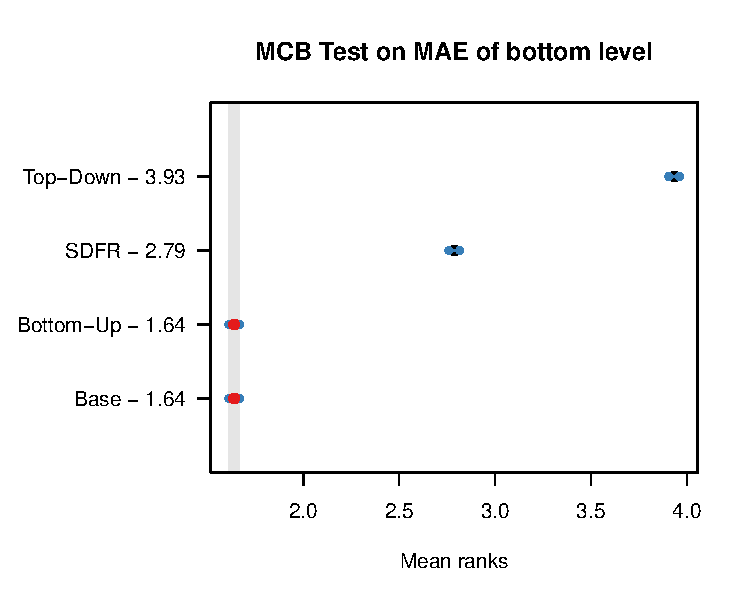
\includegraphics[width=0.45\textwidth]{figures/temporal_mcb_MAE_bottom.pdf}}
  \qquad
  \subfloat{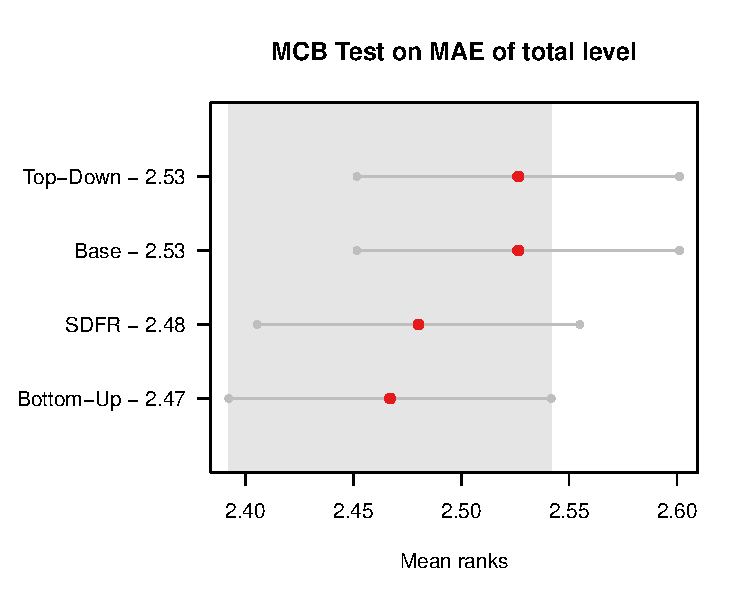
\includegraphics[width=0.45\textwidth]{figures/temporal_mcb_MAE_total.pdf}} \\

  \subfloat{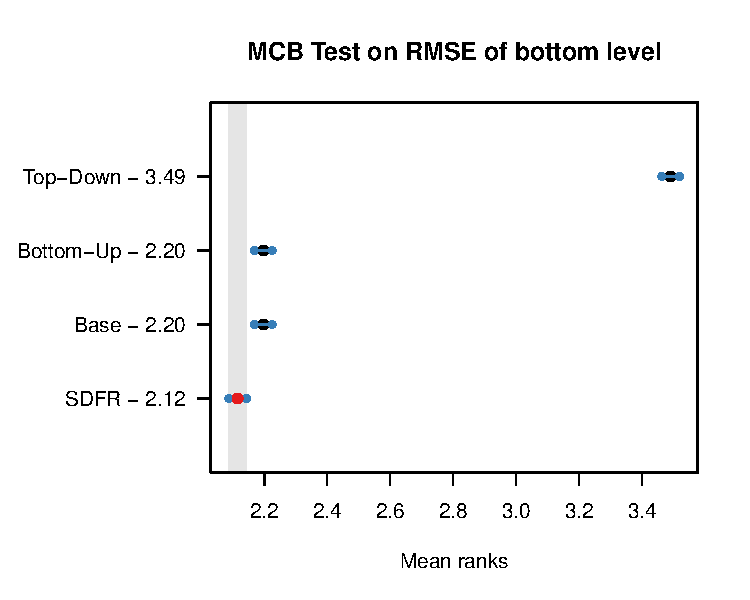
\includegraphics[width=0.45\textwidth]{figures/temporal_mcb_RMSE_bottom.pdf}}
  \qquad
  \subfloat{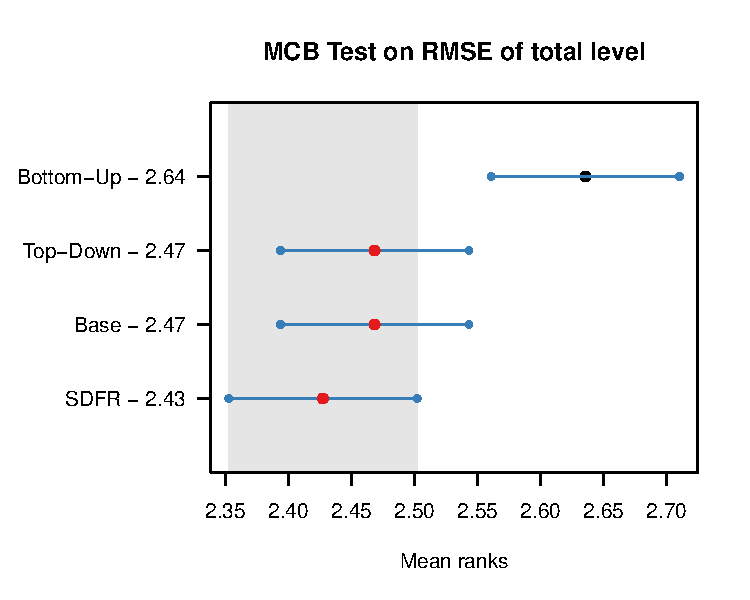
\includegraphics[width=0.45\textwidth]{figures/temporal_mcb_RMSE_total.pdf}}
\end{figure}

\begin{figure}
  \caption{\label{fig:sim_temporal_mcb_prob}MCB test of probabilistic forecasts conducted on stepwise reconciliation model in temporal setting. A 95\% confidence level is used.}
  \subfloat{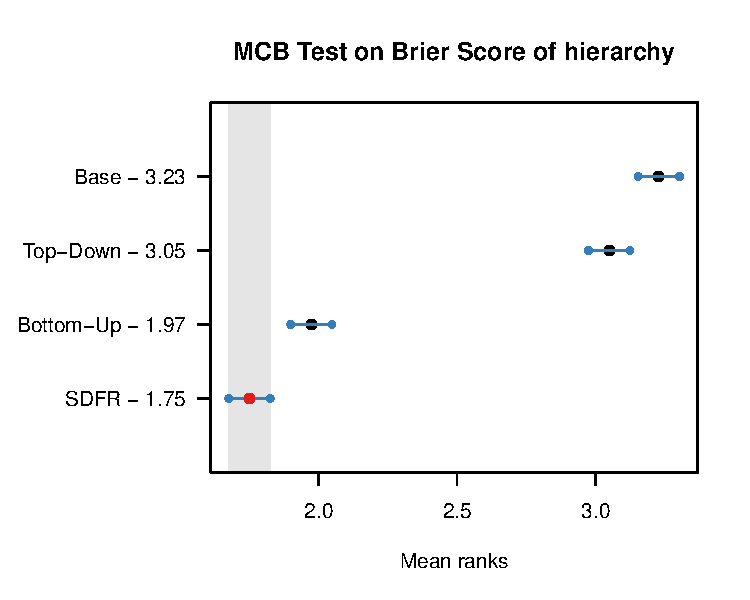
\includegraphics[width=0.32\textwidth]{figures/temporal_mcb_BS_hierarchy.pdf}} \qquad
  \subfloat{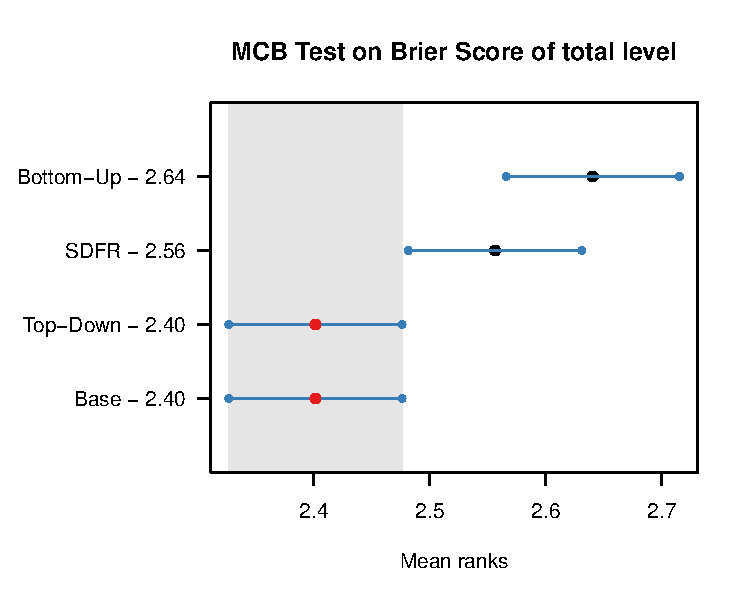
\includegraphics[width=0.32\textwidth]{figures/temporal_mcb_BS_total.pdf}} \qquad
  \subfloat{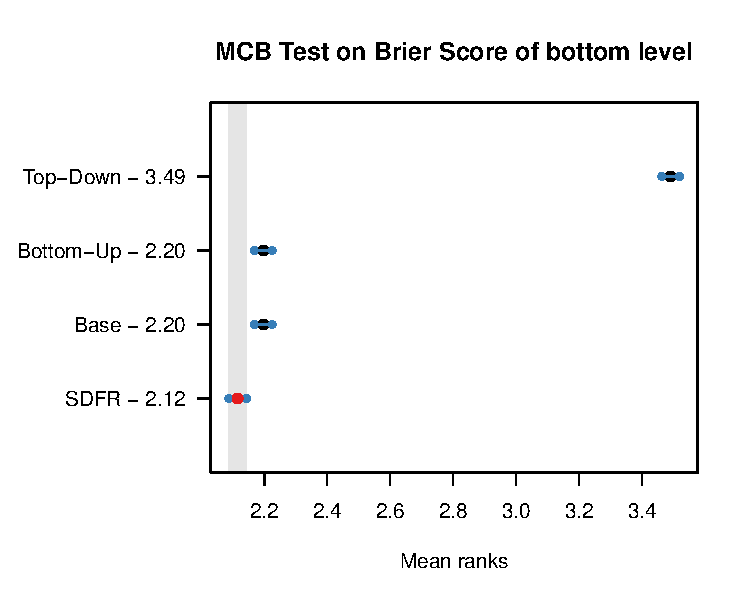
\includegraphics[width=0.32\textwidth]{figures/temporal_mcb_BS_bottom.pdf}}
\end{figure}


\section{Application: forecasting crime in Washington D.C.}
\label{sec:applications}

We apply our method to forecast offense crime case number in Washington D.C. The original dataset\footnote{The dataset can be downloaded from \url{https://crimecards.dc.gov/}} containing all crimes cases from 2014 to 2022 in Washington D.C. is aggregated into weekly time series according to location and crime type of the crime cases. 
Considering the domain of the crime number, we perform experiment on all time series whose location type is census tract and crime type is offense.
The resulted dataset includes $231$ weekly time series; each corresponds to the number of offense crimes at one census tract.

The crime time series is potentially autocorrelated (\citealp{aldor-noimanSpatioTemporalLowCount2013}). Thus, we aim to obtain coherent probabilistic crime number forecasts for next four weeks, by constructing a two-level temporal hierarchy, i.e., weekly and four-weekly, for each census tract. These two levels are referred to bottom level and total level in the rest of this section. We also constrain the maximum of the domain. For each census tract, if the max observation is $1$, then the domain is set to $[0, 1]$. Otherwise, the domain is set to $[0, 1, 2]$. The observation bigger than $2$ is set to $2$. We notice that there are less than $1\%$ of observations bigger than $2$. The modification thus has little impact on the final results.

We adopt the rolling origin strategy to train and evaluate our discrete reconciliation model. Beginning with a time series of $53$ weeks, we produce four-step-ahead probabilistic forecasts using INGARCH(3, 4). Then we increase the training data by one observation and produce new probabilistic forecasts. 
For each window, the probabilistic forecasts for total level are obtained by first aggregating weekly series into four-weekly time series, and then producing one-step-ahead forecast using INGARCH(2, 2).
The windows whose forecast horizon starts before $2022$ are used as train samples. Other windows are used to evaluate the performance.

The procedure above is repeated for each census tract. Finally, we obtain $3696$ ($231$ census tracts $\times$ $16$ test samples for each census tract) temporal hierarchies and their reconciled forecasts to evaluate the performance. The mean and median of Brier Score for total level, bottom level and the hierarchy are shown in Table~\ref{tab:crime_bs}. We also perform the MCB Test to indicate the significance of the difference.


\begin{table}[h]
  \centering
  \caption{\label{tab:crime_bs} Brier Score($\times 10^{-2}$) of test samples in crime forecasting application.}
  \begin{tabular}{ccccccccc}
  \toprule
  &\multicolumn{4}{c}{Mean} 
  & \multicolumn{4}{c}{Median} \\ \cmidrule(lr){2-5} \cmidrule(lr){6-9}
  Series & Base & Bottom-Up & Top-Down & DFR &  Base & Bottom-Up & Top-Down & DFR \\\midrule
  Total & 58.47 & \textbf{58.07} & 58.47 & 58.12 & 66.64 & 65.28 & 66.65 & \textbf{64.75} \\
  Bottom & 34.41 & 34.41 & 34.80 & \textbf{34.30} & 13.73 & 13.73 & 13.28 & \textbf{10.82}\\
  Hierarchy & 73.87 & \textbf{67.87} & 68.33 & 67.97 & 97.66 & 92.70 & 93.08 & \textbf{92.42}\\
  \bottomrule
  \end{tabular}
  \end{table}

\begin{figure}[h]
  \centering
  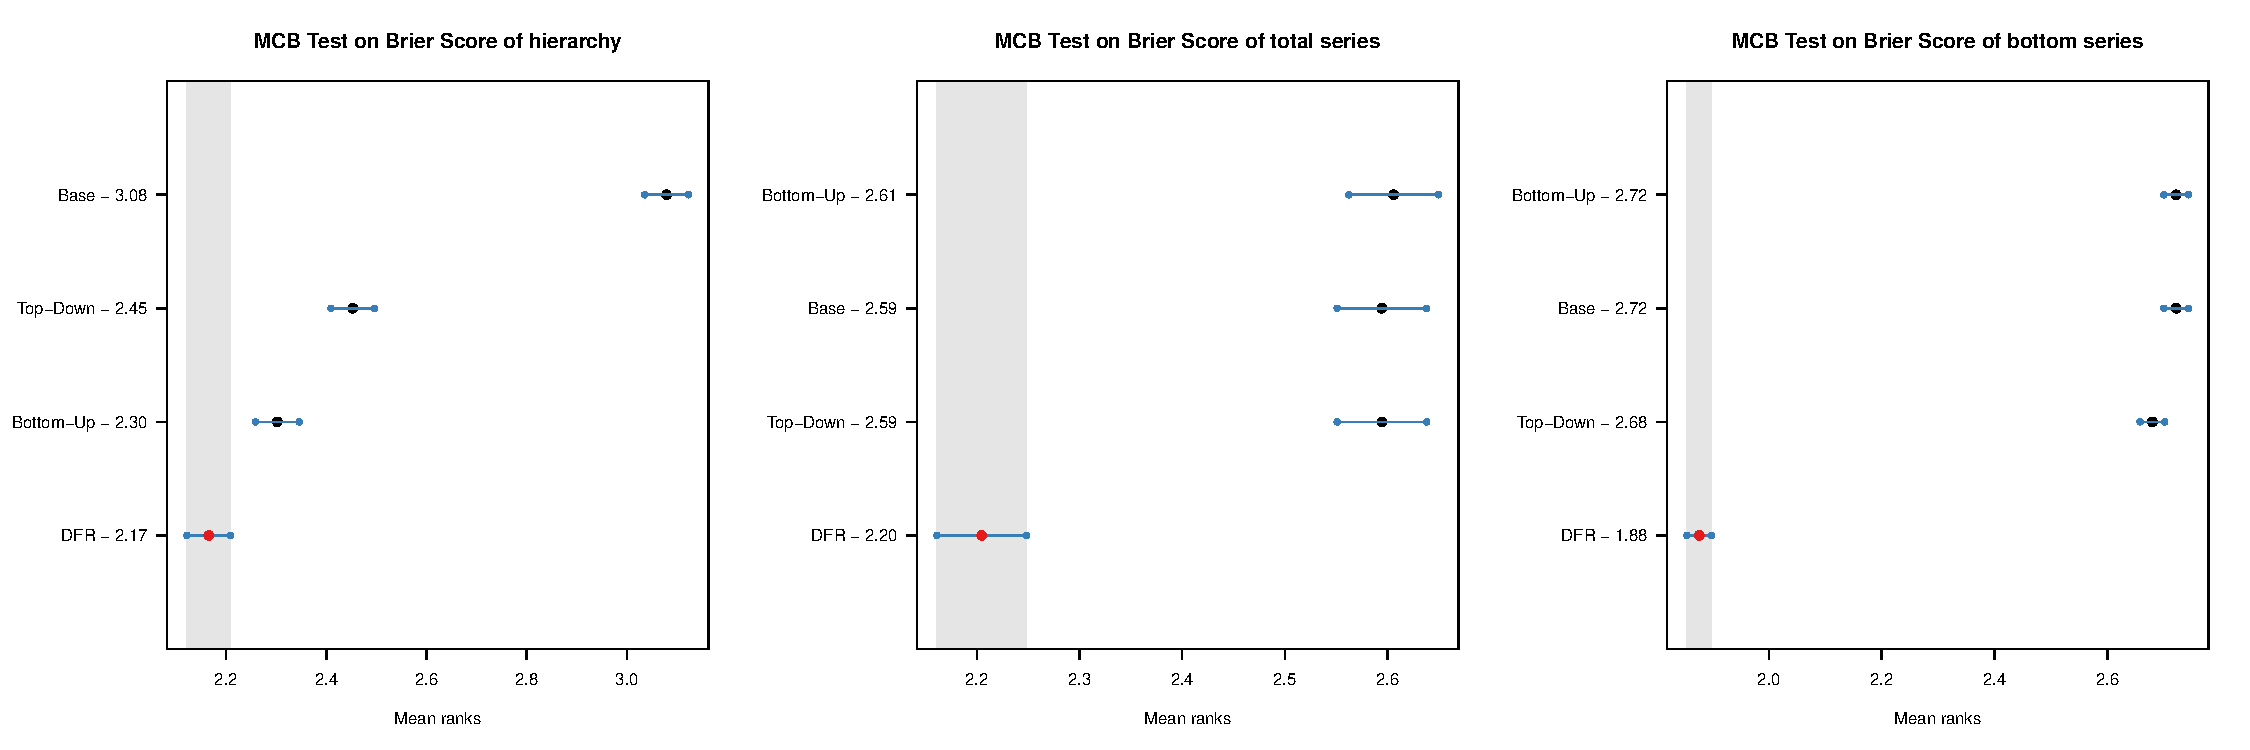
\includegraphics[width=\textwidth]{figures/dc_crime_bs.pdf}
\end{figure}

\section{Application: mortality}

The dataset contains yearly mortality data of Australia from 1921 to 2020.

\begin{enumerate}
  \item Compute the ``expected death rate'' (threshold) by asumming it decreases linearly. $l_1 - (l_{11} - l_1)/10$. (Setting2: threshold = $1.005 \times (l_1 - (l_{11} - l_1) / 10)$)
  \item If the death rate of this year is smaller than ``expected death rate'', $y$ is set to $1$.
  \item Construct the total series through aggregation.
  \item Forecast the count time series and build reconciliation model.
  \item Rolling origin strategy constructs 69 samples (1952-2020). 59 of them are used to train the model and 10 of them are used for testing.
\end{enumerate}

\begin{table}[h]
  \centering
  \caption{\label{tab:mortality_age} Probabilistic forecast performance summary of age hierarchy.}
  \begin{tabular}{ccccc}
  \toprule
  \multicolumn{5}{c}{Brier Score ($\times 10^{-3}$)}\\ 
  Serier & Base & Bottom-Up & Top-Down & DFR \\\midrule
  Total & 771.2 & 766.1 & 771.2 & \textbf{739.8} \\
  55-65 & 557.9 & 557.9 & 596.3 & \textbf{554.8} \\
  65-74 & 389.9 & 389.9 & \textbf{226.7} & 238.7\\
  75-84 & 536.6 & 536.6 & 693.3 & \textbf{311.3}\\
  85+ & \textbf{452.8}& \textbf{452.8} & 512.3 & 486.8\\
  Hierarchy & 985.3 & 936.7 & 1005.6 & \textbf{918.6} \\
  \bottomrule
  \end{tabular}
\end{table}


\begin{table}[h]
  \centering
  \caption{\label{tab:mortality_age2} Probabilistic forecast performance summary of age hierarchy (Setting 2).}
  \begin{tabular}{ccccc}
  \toprule
  \multicolumn{5}{c}{Brier Score ($\times 10^{-3}$)}\\ 
  Serier & Base & Bottom-Up & Top-Down & DFR \\\midrule
  Total & 638.0 & 626.7 & 638.0 & \textbf{590.8} \\
  55-65 & \textbf{174.5} & \textbf{174.5} & 203.3 & 175.1 \\
  65-74 & 138.3 & 138.3 & 142.9 & 128.9\\
  75-84 & 205.5 & 205.5 & 324.4 & \textbf{160.4}\\
  85+ & 495.3 & 495.3 & \textbf{444.2} & 521.6\\
  Hierarchy & 882.4 & 697.0 & 736.7 & \textbf{675.2} \\
  \bottomrule
 \end{tabular}
\end{table}

\section{Conclusion}
\label{sec:conclusion}

\newpage

\appendix
\section{Adjust algorithm}
\label{appendix:adjust}


\newpage

\bibliographystyle{agsm}
\bibliography{references.bib}

\end{document}